\section{Trigger and Preselection}\label{sec:ggtt_trigger_preselection}

Events from data-taking periods that are certified for physics events are first selected according to HLT paths that require two photons that pass a set of criteria on the \pt of the photons and the invariant mass of the diphoton system. The HLT path used in the low-mass \XYggHtt search requires $\mgg > 55$\GeV and $\pt > 30 (18)$\GeV for the leading (subleading) photon. The HLT path used for all of the other searches in this analysis requires $\mgg > 90$\GeV and has the same photon \pt requirements except in 2017 and 2018 where the subleading photon threshold was increased to 22\GeV. The HLT paths also apply a set of loose requirements on shower shape and isolation variables of the photons. The impact of including tau lepton triggers was studied, but the improvement in signal efficiencies was found to be less than 1\% and therefore, these triggers were not used in the final analysis.

Triggered events are then required to pass a set of preselection criteria. This selection requires tau lepton candidates in the event, applies the particle identification algorithms described in \cref{sec:reconstruction}, and places loose requirements on kinematic properties of the photons and tau lepton candidates. Selections are also placed on a number of shower shape and isolation variables for the photons: \Ich, H/E, \RNINE, $\sigma_{i\eta i\eta}$ and \Iph (all defined in \cref{sec:eg_id}), and on impact parameters \dxy and \dz, which are the shortest distances of the corresponding particle track to the primary vertex in the transverse and longitudinal directions respectively.

The preselection requirements are kept as loose as possible, either aligning with the trigger (HLT) requirements, which were originally tuned to maximize the signal efficiency for SM \PH production for a particular trigger rate/bandwidth, or aligning with requirements used to derive simulation corrections, e.g.\ the electron ID efficiency scale factors (\cref{sec:eg_id}) were calculated for electrons with $\pt>10$\GeV. Later, the pNN will be used to apply the final selection designed to optimize the sensitivity of the analysis. 

Beginning with the photons, the preselection requirements depend on which search is being performed where different requirements are made for the low-mass \XYggHtt search compared to the rest of the searches. Starting with the requirements for the rest of the searches, all photon candidates are required to have:
\begin{itemize}
  \setlength{\itemsep}{-3pt}
  \item $\pt > 25\GeV$,
  \item $\abs{\eta} < 2.5$ and not $1.44 < \abs{\eta} < 1.57$ (to exclude the barrel-endcap transition region),
  \item $\Ich < 20$\GeV,
  \item $\Ich / \pt^\gamma < 0.3$,
  \item $\text{H/E} < 0.08$, 
  \item Photon ID WP90
\end{itemize} 
and pass additional $\eta$-dependent requirements on \RNINE, $\sigma_{i\eta i\eta}$ and \Iph, which are summarized in \cref{tab:photon_preselection}. These requirements also include a selection on track isolation, \Itk, which is the sum of track \pt in a hollow cone with a smaller (larger) annulus of ${\Delta}R=0.04\ (0.33)$. For the \XHH and \XYttHgg searches, diphoton candidates are then formed by pairing photons that have $100 < \mgg < 180$\GeV and where the leading (subleading) photon has $\pt > 35\,(25)$\GeV. Additionally, the leading (subleading) photon is required to have $\pt / \mgg > 0.33\, (0.25)$. The same requirements are applied in the high-mass \XYggHtt search except the \mgg requirement is changed to $100 < \mgg < 1000$\GeV.

\begin{table}
  \centering
  \caption[$\eta$-dependent Preselection Requirements]{A subset of the preselection requirements on photon candidates that are based upon $\eta$, \RNINE, $\sigma_{i\eta i\eta}$, \Iph, and \Itk.}\label{tab:photon_preselection}

  \begin{tabular}{ccccc}
    \toprule
                             & \RNINE       & $\sigma_{i\eta i\eta}$ & \Iph (\GeV) & \Itk (\GeV) \\
    \midrule
    \multirow{2}{*}{Barrel}  & [0.50, 0.85] & $<$0.015               & $<$4.0                    &  $<$6.0                   \\
                             & $>$0.85      &          ---           & ---                       &---                        \\
    \multirow{2}{*}{Endcaps} & [0.80, 0.90] & $<$0.035               & $<$4.0                    &  $<$6.0                   \\
                             & $>$0.90      &          ---           & ---                       &---                        \\
  \bottomrule
  \end{tabular}
\end{table}  

In the low-mass search, the \pt requirement on photon candidates is lowered to 18\GeV, and the pixel veto (\cref{sec:eg_reco}) is applied to reduce contamination from the DY background. All other photon requirements are the same. When forming diphoton candidates, the leading (subleading) photon is required to have $\pt > 30$ (18)\GeV, the $\pt / \mgg$ requirements are removed, and $65 < \mgg < 150$\GeV is required. In all searches, if more than one diphoton candidate is found, the candidate with the highest \pt is chosen.

\begin{table}
  \centering
  \caption[Preselection Requirements for Electrons, Muons, \tauh, and Jets]{Preselection requirements on electrons, muons, \tauh, and jets. Descriptions about the ID algorithms for electrons, muons and \tauh can be found in \cref{sec:reconstruction}. In addition to the listed criteria, selected electrons, muons and \tauh are required to have $\dR > 0.2$ with respect to each other and selected photons, and jets are required to have $\dR > 0.4$ with respect to all selected objects. Finally, electrons whose trajectories are consistent with the barrel-endcap transition region ($1.44 < \abs{\eta} < 1.57$) are excluded.}\label{tab:preselection_other_objects}
  \renewcommand{\arraystretch}{1.2}
  \begin{tabular}{@{}lccccl@{}}
  \toprule
            & \pt     & \abseta & \absdxy & \absdz & ID                                          \\ \midrule
  Electrons & >10\GeV & <2.5    & <0.045  & <0.2   & WP90                                        \\
  Muons     & >15\GeV & ---     & <0.045  & <0.2   & Medium cut-based                            \\
  \tauh     & >20\GeV & <2.3    & ---     & <0.2   & VVLoose \De, VLoose \Dm, Loose \Djet \\ 
  Jets      & >25\GeV & <2.4    & ---     & ---    & ---                                         \\ 
  IsoTracks & >5\GeV & --- & <0.2 & <0.1 & --- \\
  \bottomrule
  \end{tabular}
\end{table}

Electron, muon, \tauh, and jet candidates are selected according to the criteria summarized in \cref{tab:preselection_other_objects}. This includes selection on the candidate \pt, \eta, ID variables, and the impact parameters, \dxy and \dz, which are the shortest distances of the track to the primary vertex in the transverse and longitudinal directions respectively. 

Ditau candidates are formed by creating pairs of candidates from the selected \tauh, muon, electron candidates according to the following priority: $\tauh\tauh$, $\tauh\mu$, $\tauh e$, $\mu e$, $\mu\mu$, $ee$, where a particular pairing is referred to as a channel. If there is one \tauh candidate, and no electron or muon candidates, tracks with $\Ich < 5$\GeV and $\pt > 5$\GeV, or $\Ich / \pt < 0.2$ are considered as additional tau lepton candidates. These isolated tracks (IsoTracks) are used to create an additional channel: $\tauh + \text{IsoTrack}$. Events are selected if they have a ditau candidate, or if there is a single \tauh, which is the final channel: $\tauh$.

Events with an opposite-sign same flavour $ee$ or $\mu\mu$ pair are rejected if they are consistent with a $Z \to ll$ or $Z \to ll\gamma$ ($l = e, \mY$) decay. This is done by rejecting any events where $80 < m_{ll} < 100$\GeV or $86 < m_{ll\gamma} < 96$\GeV where $m_{ll\gamma}$ is calculated with respect to both the leading and subleading photons.

The efficiency of the triggering and preselection requirements for signal events is calculated in simulation with a number of corrections applied. These corrections include the object energy scale, energy resolution, and ID corrections discussed in \cref{sec:reconstruction}. They also include corrections for the triggering and photon preselection requirements which are derived from data with the ``tag-and-probe'' method using \Zee events~\cite{CMS:2011aa}, and are applied by reweighting the simulated events in bins of \pt, \RNINE and \eta~\cite{CMS:2018piu,CMS:2020xrn,CMS:2021kom}.

The signal efficiency after triggering and preselection requirements is shown as a function of the resonance mass, \mX, for the \XHH searches in \cref{fig:presel_eff_graviton}, which is seen to increase as a function of \mX. This is expected since a higher \mX will lead to candidates with higher \pt, which will be more likely to pass the \pt requirements. Furthermore, the efficiency of ID requirements tend to increase with higher \pt (see \cref{fig:tau_reco_id_eff}). 

\begin{figure}
  \centering
  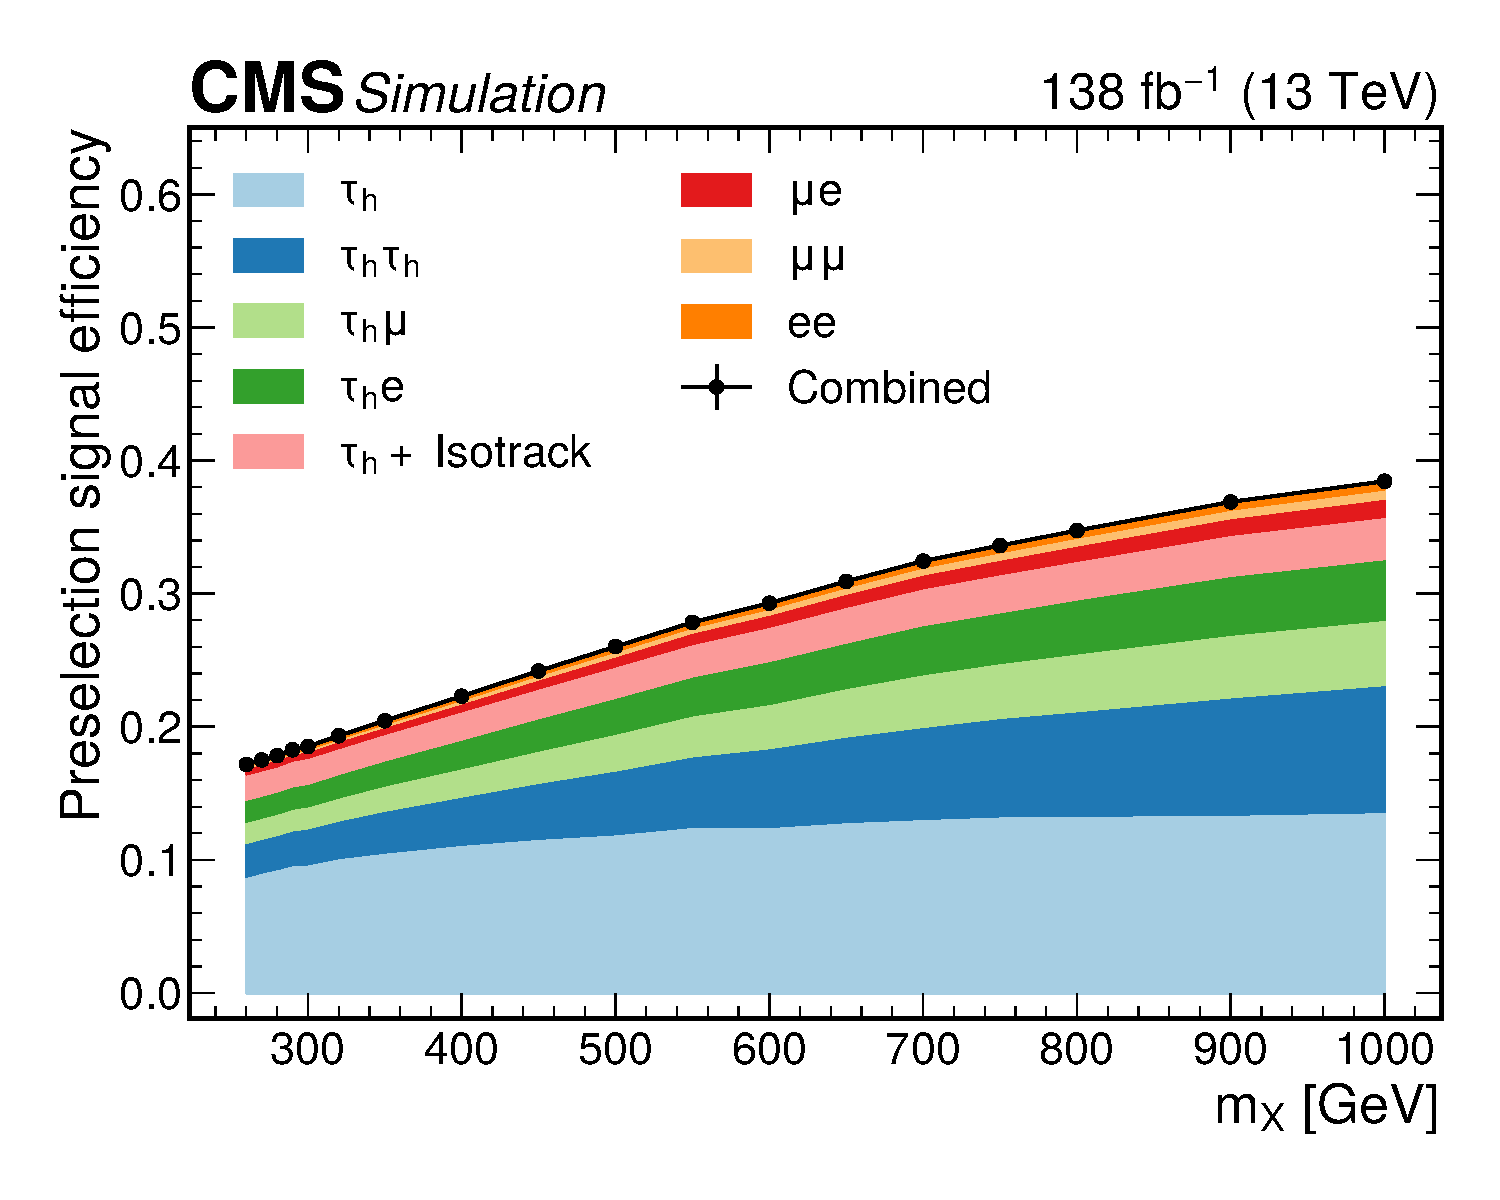
\includegraphics[width=.49\linewidth]{Figures/Dihiggs/trigger/Radion/sig_eff_stack_thesis.pdf}
  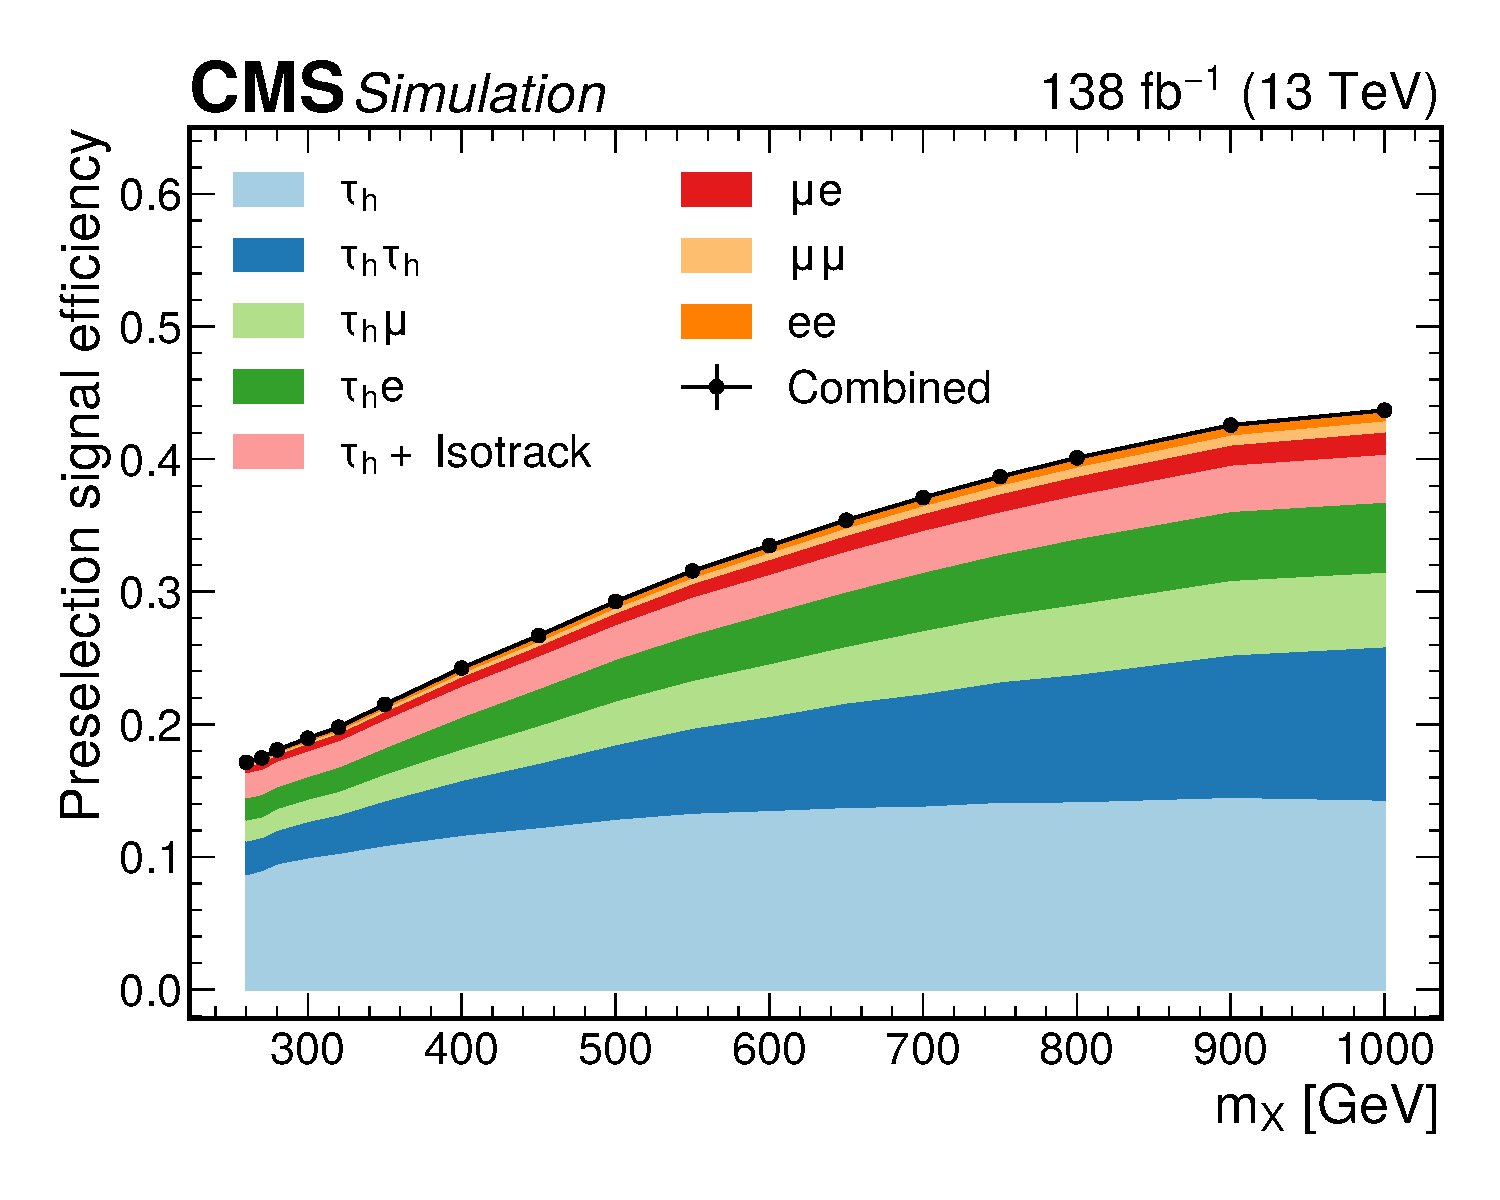
\includegraphics[width=.49\linewidth]{Figures/Dihiggs/trigger/Graviton/sig_eff_stack_thesis.pdf}
  \caption[Preselection Efficiency as a Function of \mX in the \XHH Searches]{Preselection signal efficiency as a function of \mX in the \XZeroHH (left) and \XTwoHH(right) searches. The contributions from the different channels are shown by the stacked filled histograms and the combined efficiency shown by the black points. The statistical uncertainty in the combined uncertainty is plotted but is too small to be seen.}\label{fig:presel_eff_graviton}
\end{figure}

The preselection efficiency in the \XYH searches is shown in \cref{fig:presel_eff_xyh} as functions of \mX and \mY. As in the \XHH searches, the efficiency increases with \mX. In the high-mass \XYggHtt search, the trend in \mY is such that the highest efficiencies are found at low \mY, whereas in the low-mass search less of a significant trend is seen, though that is likely due to the smaller range of \mY being considered. In the \XYttHgg search, a more complex trend in \mY is seen, where the highest efficiencies are seen for median values of \mY. The is possibly because at lower values of \mY, the tau lepton candidates will be less separated and the \dR requirement between tau lepton candidates will reduce the efficiency.

\begin{figure}
  \centering
  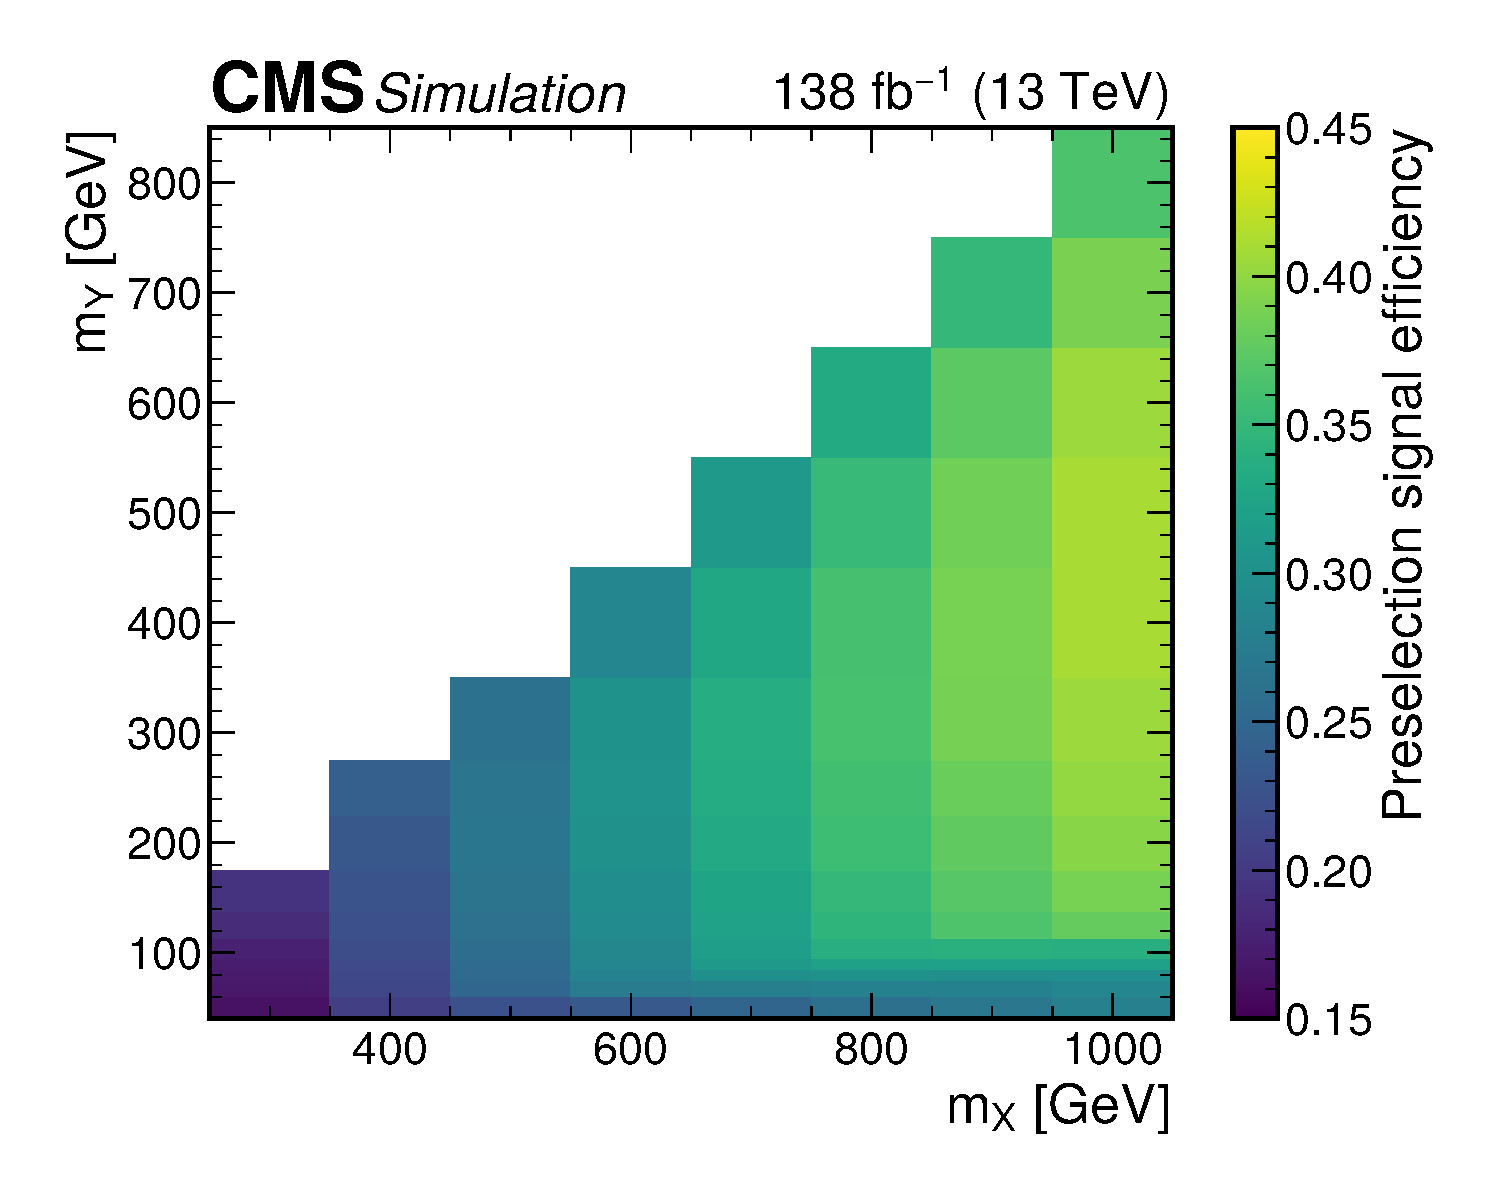
\includegraphics[width=.49\linewidth]{Figures/Dihiggs/trigger/Y_tautau/sig_eff_heatmap_thesis.pdf} \\
  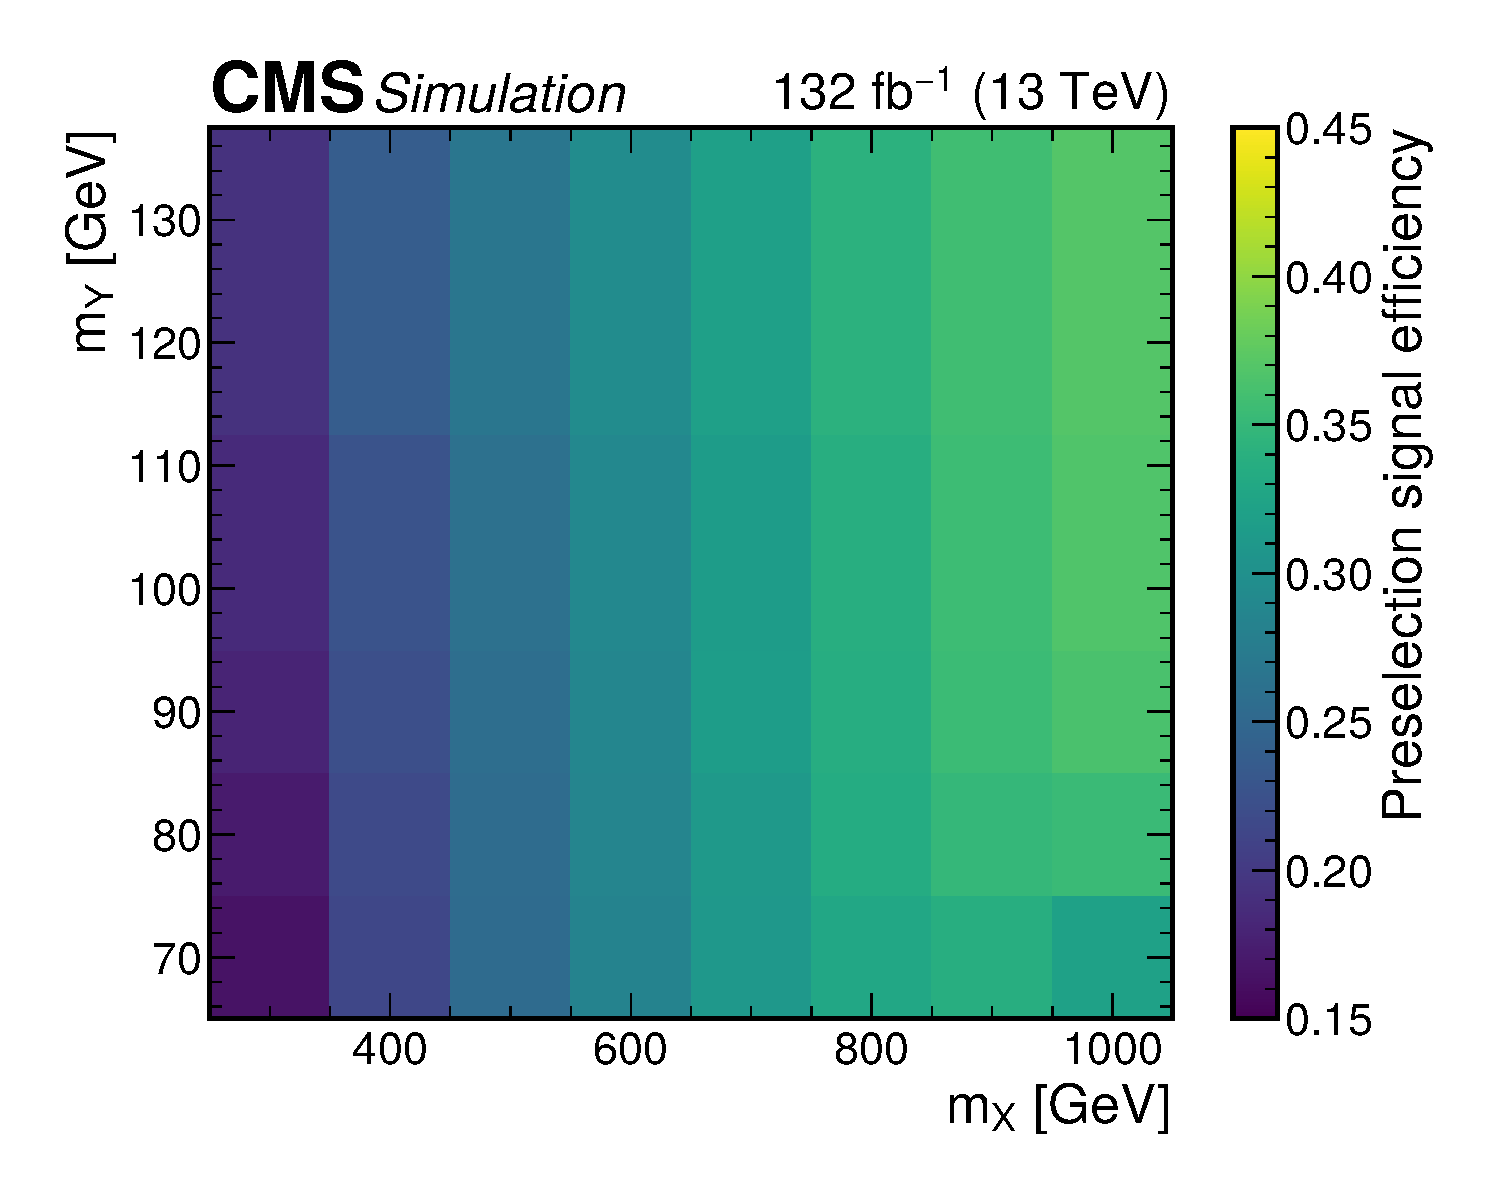
\includegraphics[width=.49\linewidth]{Figures/Dihiggs/trigger/Y_gg_Low_Mass/sig_eff_heatmap_thesis.pdf}
  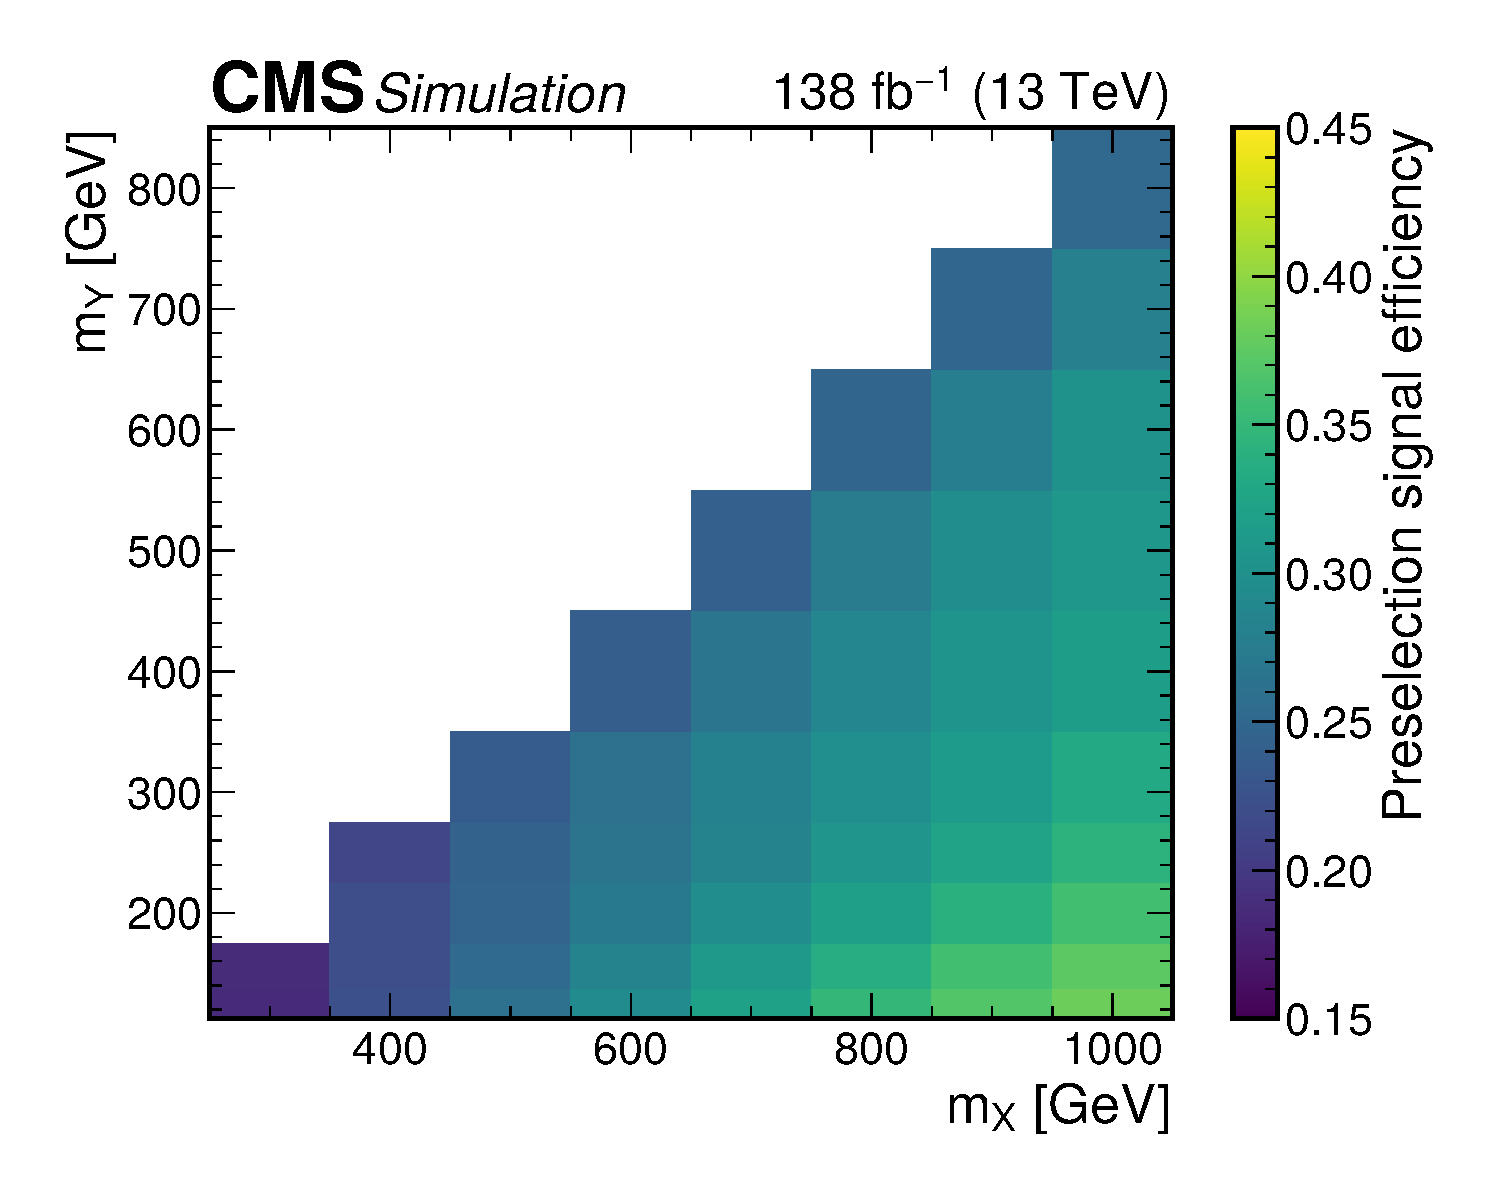
\includegraphics[width=.49\linewidth]{Figures/Dihiggs/trigger/Y_gg_High_Mass/sig_eff_heatmap_thesis.pdf}
  \caption[Preselection Efficiency as a Function of \mX and \mY in the \XYH Searches]{Preselection signal efficiency as a function of \mX and \mY in the \XYttHgg (top), low-mass \XYggHtt (bottom-left), and high-mass \XYggHtt (bottom-right) searches.}\label{fig:presel_eff_xyh}
\end{figure}
